%!TEX root = ../../csuthesis_main.tex
\chapter{算法仿真实验}

\section{任务计算资源调度算法仿真实验}

为验证任务计算资源调度算法ASA和FD的有效性和优越性,本节完成并应用了任务生成器来随机生成包含着任务起始时间、所需计算资源、在不同设备上的计算时间、上传时延等的任务数据,并与采用了与ASA算法相同的邻域结构的SA算法进行测试对比。

\subsection{参数设置}

在设置任务生成器的参数时,本节使用了表~\ref{tab:资源分配算法任务生成参数}中的参数来生成近似真实应用场景下的计算型任务数据,其中任务总数\( N \)为50,每个任务的起始时间\(S_i\)为上下界分别为1000、0的离散型均匀分布,每个任务的计算所需资源\(R_i\)为上下界分别为100、1的离散型均匀分布,每个任务在无人机上计算需要花费的时间\(U_i\)为上下界300、1的离散性均匀分布,每个任务在服务器上计算需要花费的时间\(C_i\)为上下界\(U_i-1\)、0的离散性均匀分布,上传时延\(D_i\)为上下界100、1的离散型均匀分布。

\begin{table}[!htbp]
    \caption{资源分配算法任务生成参数}
    \label{tab:资源分配算法任务生成参数}
    \centering
    \begin{tabular}{c c c}
        \toprule
        \textbf{参数} & \textbf{含义} & \textbf{值}\\
        \midrule
        \( N \) & 任务总数 & 50 \\
        \( S_i \) & 第\(i\)个任务的起始时间 & \([0, 1000]\) \\
        \( R_i \) & 第\(i\)个任务所花费的资源 & \([1, 100]\) \\
        \( U_i \) & 第\(i\)个任务在无人机上计算需要花费的时间 & \([1, 300]\) \\
        \( C_i \) & 第\(i\)个任务在服务器上计算需要花费的时间 & \([0, U_i-1]\) \\
        \( D_i \) & 第\(i\)个任务上传至其他设备的时延 & \([1, 100]\) \\
        \bottomrule
    \end{tabular}
\end{table}

\begin{table}[!htbp]
    \caption{任务计算资源调度算法实验参数设置}
    \label{tab:任务计算资源调度算法实验参数设置}
    \centering
    \begin{tabular}{c c c}
        \toprule
        \textbf{参数} & \textbf{含义} & \textbf{值}\\
        \midrule
        \( N_u \) & 无人机数量 & 30 \\
        \( R_u \) & 无人机最大可用计算资源 & 100 \\
        \( N_c \) & 服务器数量 & 1 \\
        \( R_c \) & 服务器最大可用计算资源 & 2000 \\
        \bottomrule
    \end{tabular}
\end{table}


测试中采用的实验参数如表~\ref{tab:任务计算资源调度算法实验参数设置}所示,其中无人机的数量\( N_u \)为30,每架无人机最大可用的计算资源\(R_u\)为100,服务器的数量\( N_c \)为1,每台服务器最大可用的计算资源\( R_c \)为2000。

\begin{table}[!htbp]
    \caption{算法参数设置}
    \label{tab:算法参数设置}
    \centering
    \begin{tabular}{c c c c c c}
        \toprule
        \multicolumn{3}{c}{\textbf{SA}} & \multicolumn{3}{c}{\textbf{ASA}} \\
        \cmidrule(lr){1-3} \cmidrule(lr){4-6} 
        参数 & 含义 & 值 & 参数 & 含义 & 值\\
        \midrule
        \( T_{\textrm{init}} \) & 初始温度 & 1,000 & \( N \) & 总迭代次数 & 1000 \\
        \( T_{\textrm{end}} \) & 终止温度 & 1 & \( T_{\textrm{min}} \) & 最低温度 & 1 \\
        \( \rho_{\textrm{cool}} \) & 冷却速率 & 0.9 & \( \rho \) & 升温速率 & 1 \\
        \( n_T \) & 每个温度下的迭代次数 & 15 & \( \delta \) & 温控参数 & 0.01 \\
        \bottomrule
    \end{tabular}
\end{table}

本文所提出的ASA算法以及对比算法SA的参数设置如表~\ref{tab:算法参数设置}所示,即对于SA来说,其初始温度\( T_{\textrm{init}} \)为\(10^4\),终止温度\( T_{\textrm{end}} \)为\(10^{-1}\),冷却速率\( \rho_{\textrm{cool}} \)为0.9,每个温度下的迭代次数\(n_T\)为10,而对于ASA来说,其总迭代次数\(N\)为1000,最低温度\(T_{\textrm{min}}\)为1,升温速率\( \rho \)为1,温控参数\( \delta \)为1。

\subsection{算法性能对比实验结果}

为了能够直观地体现ASA算法的有效性及优越性,本节统计了十次性能测试的性能指标,其具体的性能结果如表~\ref{tab:资源分配算法性能比较结果}所示。

\begin{table}[!htbp]
    \caption{资源分配算法性能比较结果}
    \label{tab:资源分配算法性能比较结果}
    \centering
    \begin{tabular}{c c c c c c c}
        \toprule
        \multirow{2}{*}{\textbf{测试数据}} & \multicolumn{2}{c}{\textbf{SA}} & \multicolumn{2}{c}{\textbf{ASA}} & \multicolumn{2}{c}{\textbf{FD}}\\
        \cmidrule(lr){2-3} \cmidrule(lr){4-5} \cmidrule(lr){6-7}
        & \makecell{运行时间\\(秒)} & 目标值 & \makecell{运行时间\\(秒)} & 目标值 & \makecell{运行时间(秒)} & 目标值 \\
        \midrule
        1 & 203.324 & 30372 & 198.497 & 30313 & 0.038 & 30480\\
        2 & 223.149 & 29809 & 177.082 & 29809 & 0.039 & 29809\\
        3 & 216.077 & 31359 & 174.673 & 31359 & 0.039 & 31408\\
        4 & 234.679 & 31732 & 172.580 & 31686 & 0.041 & 32188\\
        5 & 227.150 & 31067 & 197.496 & 30597 & 0.040 & 31116\\
        6 & 238.868 & 30780 & 185.066 & 30888 & 0.041 & 31272\\
        7 & 209.149 & 31986 & 187.116 & 31309 & 0.042 & 31986\\
        8 & 252.184 & 32551 & 179.438 & 32467 & 0.041 & 32683\\
        9 & 221.427 & 29638 & 179.438 & 29152 & 0.039 & 29915\\
        10 & 195.529 & 30699 & 160.609 & 30606 & 0.040 & 30883\\
        \textbf{平均值} & 222.238 & 30956.4 & 184.156 & \textbf{30818.6} & \textbf{0.040} & 31174\\
        \bottomrule
    \end{tabular}
\end{table}

根据表~\ref{tab:资源分配算法性能比较结果}的试验结果,在目标值方面,本文所提出的ASA算法相较其他对比算法,得到的解质量更好,这体现了ASA算法在解决无人机任务执行开始前的任务计算资源调度静态问题时的有效性;在运行时间方面,ASA算法相较于SA算法有着更少的算法运行时间,同时FD算法的运行时间与其他算法的运行时间更是有着明显的差距,而FD算法虽然得到的解的质量较差,但由于其用于无人机任务执行开始后的动态问题,相较于目标性能,其运行时间更为重要。因此本文的ASA算法与FD算法在该问题下的优越性明显。

\section{静态场景下的无人机航迹规划算法仿真实验}

为验证本文所提出的静态场景下的无人机航迹规划算法RRT*-Connect的有效性及优越性,本节完成并应用了地图生成器来随机生成包含着不同障碍物、起终点的地图信息进行测试,并与其他同样能够用于航迹规划的Basic RRT算法、基于概率的RRT算法、RRT-Connect以及RRT*算法进行测试比较。

\subsection{仿真参数设置}

在设置地图生成器的参数时,本节使用了表~\ref{tab:航迹规划算法仿真环境参数}中的参数来生成近似真实城市环境的三维地图,其中该地图的大小为\( B_x \times B_y \times B_z \),每个位置的生成建筑物的概率\( P_b \)为10\%,建筑物的高度分布为均值\( \mu = B_z / 2\)的均值分布,建筑物所占地面面积\( S_b \)为固定为1,共生成\( N \)个测试地图。

\begin{table}[!htbp]
    \caption{静态场景下的无人机航迹规划算法仿真环境参数}
    \label{tab:航迹规划算法仿真环境参数}
    \centering
    \begin{tabular}{c c c}
        \toprule
        \textbf{参数} & \textbf{含义} & \textbf{值}\\
        \midrule
        \(B_x\) & 地图在\(x\)轴上的长度 & \(100\) \\
        \(B_y\) & 地图在\(y\)轴上的长度 & \(100\) \\
        \(B_z\) & 地图在\(z\)轴上的长度 & \(10\) \\
        \(P_b\) & 建筑物的生成概率 & \(10\%\)\\
        \( \mu \) & 建筑物高度的分布均值 & \(50\) \\
        \( S_b \) & 建筑物所占地面面积 & \(1\) \\
        \(N\) & 进行测试的地图数量 & \(100\) \\
        \bottomrule
    \end{tabular}
\end{table}

本文提出的RRT*-Connect算法与对比算法Basic RRT算法、基于概率的RRT算法、RRT-Connect算法与RRT*算法均采用相同的参数设置,即表~\ref{tab:无人机航迹规划算法参数设置}中所示,即对于上述每一个算法生成的随机树来说,其可容许的最大的步进拓展的长度\(S\)为1,在对地图进行采样时选取目标点的概率\(P_t\)为0.2。

\begin{table}[!htbp]
    \caption{静态场景下的无人机航迹规划算法参数设置}
    \label{tab:无人机航迹规划算法参数设置}
    \centering
    \begin{tabular}{c c c}
        \toprule
        \textbf{参数} & \textbf{含义} & \textbf{值}\\
        \midrule
        \( S \) & 步进长度 & 1\\
        \( P_t \) & 采样时选取目标点的概率 & 0.2\\
        \bottomrule
    \end{tabular}
\end{table}

\subsection{仿真实验结果}

为了直观地体现RRT*-Connect算法的有效性,本节选取了其中一次测试的结果并使其可视化,其建筑分布、飞行航迹等信息如图~\ref{fig:RRT*-Connect在三维地图下的仿真结果}所示,从图中可以明显看出,基于RRT*-Connect的航迹规划算法在模拟城市的三维环境下成功地躲避了环境中的建筑物,并成功地在较短航程下到达了目标点。

\begin{figure}[!htbp]
    \centering
    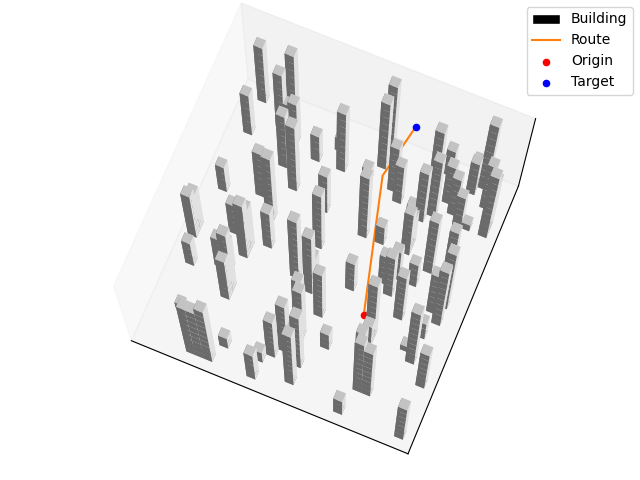
\includegraphics[width=0.75\textwidth]{./images/test_1_Connect_RRT_Star_1.png}
    \caption{基于RRT*-Connect的航迹规划算法在三维地图下的仿真结果}
    \label{fig:RRT*-Connect在三维地图下的仿真结果}
\end{figure}

\subsection{算法性能对比实验结果}

为了直观地体现RRT*-Connect算法的优越性,本节统计了性能测试中得到的性能指标,具体结果如表~\ref{tab:航迹规划算法性能比较结果}所示。

\begin{table}[!htbp]
    \caption{航迹规划算法性能比较结果}
    \label{tab:航迹规划算法性能比较结果}
    \centering
    \begin{tabular}{c c c}
        \toprule
        \textbf{算法} & \textbf{目标值} & \textbf{运行时间} \\
        \midrule
        Basic RRT & 105.313 & 4.008  \\
        基于概率的RRT & 87.878 & 3.710  \\
        RRT-Connect & 83.699 & \textbf{0.076} \\
        RRT* & 81.686 & 0.498 \\
        RRT*-Connect & \textbf{79.312} & 0.132 \\
        \bottomrule
    \end{tabular}:
\end{table}

根据表~\ref{tab:航迹规划算法性能比较结果}的试验结果,在目标值方面,本文所提出的RRT*-Connect算法相较其他对比算法,得到的解质量更好,这体现出了本文RRT*-Connect算法在解决城市密集障碍物环境下静态场景下的无人机航迹规划问题时的优越性;在运行时间方面,本文算法相较大部分对比算法而言有着更短的平均计算时间,仅相对于RRT-Connect在计算时间方面有着微小的差距,这是由于RRT*-Connect算法采用的Rewire机制导致算法计算量增加,进而造成计算时间的略微增加,但其求解结果却有了明显的提升。于此同时,由于本文研究的无人机航迹规划算法是在无人机任务执行开始之前,在服务器上运行生成航迹规划方案,相较于算法运行时间,其目标性能更为重要,因此本文的RRT*-Connect算法在该场景下的优越性更加明显。

\section{动态场景下的无人机航迹规划算法仿真实验}

为验证无人机实时避障算法A*的有效性及优越性,本节完成并应用了地图生成器来随机生成包含着不同障碍物、起终点的地图信息进行测试,并与同样能够应用于避障航迹生成的Basic RRT算法、基于概率的RRT算法、RRT-Connect、RRT*以及RRT*-Connect算法进行测试比较。

\subsection{仿真实验参数}

与静态场景下的航迹规划算法所解决的问题不同,动态场景下的无人机航迹规划算法所解决的动态场景下的无人机航迹规划问题的地图数据相对更小,且其实时性使得对算法的运行速度有着很高的要求,因此本文在设置地图生成器的参数时,为便于观察可视化结果,采用了表~\ref{tab:实时避障算法仿真环境参数}中的参数来随机生成包含不同障碍物、起终点的二维地图信息来生成算法的测试数据,其中,该地图大小为\( B_x \times B_y \),每个位置生成障碍物的概率\( P_b \)为\(10\%\),共生成\( N \)个测试地图。

\begin{table}[!htbp]
    \caption{动态场景下的无人机航迹规划算法仿真环境参数}
    \label{tab:实时避障算法仿真环境参数}
    \centering
    \begin{tabular}{c c c}
        \toprule
        \textbf{参数} & \textbf{含义} & \textbf{值}\\
        \midrule
        \(B_x\) & 地图在\(x\)轴上的长度 & \(30\) \\
        \(B_y\) & 地图在\(y\)轴上的长度 & \(30\) \\
        \(P_b\) & 障碍物的生成概率 & \(10\%\) \\
        \(N\) & 进行测试的地图数量 & \(100\) \\
        \bottomrule
    \end{tabular}
\end{table}

本文所使用的A*算法与对比算法Basic RRT算法、基于概率的RRT算法、RRT-Connect算法、RRT*算法与RRT*-Connect算法均采用相同的参数设置,即表~\ref{tab:实时避障算法参数设置}中所示,对于Basic RRT及其他基于Basic RRT的算法,采用RRT及其衍生算法下的参数,即其随机树的可容许最大步进拓展长度\(S\)为1,在对地图进行采样时选取目标点的概率\(P_t\)为0.2;对于A*算法而言,仅需设置其每一步的步进长度\(S\)为1。

\begin{table}[!htbp]
    \caption{动态场景下的无人机航迹规划算法参数设置}
    \label{tab:实时避障算法参数设置}
    \centering
    \begin{tabular}{c c c c c c}
        \toprule
        \multicolumn{3}{c}{\textbf{RRT及其衍生算法}} & \multicolumn{3}{c}{\textbf{A*}} \\
        \cmidrule(lr){1-3} \cmidrule(lr){4-6}
        参数 & 含义 & 值 & 参数 & 含义 & 值 \\
        \midrule
        \( S \) & 步进长度 & 1 & \( S \) & 步进长度 & 1 \\
        \( P_t \) & 采样时选取目标点的概率 & 0.2 & & & \\
        \bottomrule
    \end{tabular}
\end{table}

\subsection{仿真实验结果}

为了能够直观地体现A*的有效性,本节选取其中一次测试的结果并将其可视化,其障碍物分布、避障航迹如图~\ref{fig:A*算法在二维地图下的仿真结果}所示,从图中能够看出A*算法成功地根据已知障碍物信息规划出了一条能够躲避障碍物的飞行航迹。

\begin{figure}[!htbp]
    \centering
    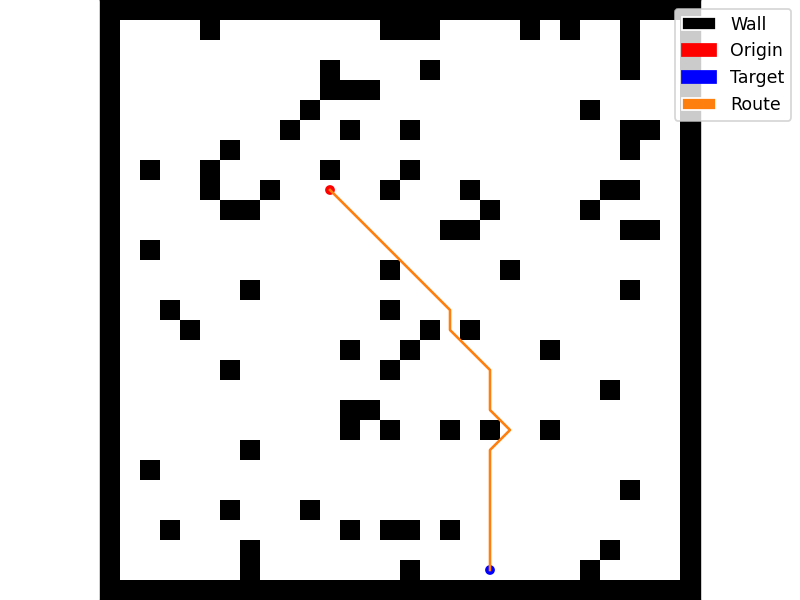
\includegraphics[width=0.65\textwidth]{images/test_8_A_Star.png}
    \caption{A*算法在二维地图下的仿真结果}
    \label{fig:A*算法在二维地图下的仿真结果}
\end{figure}

\subsection{算法性能对比实验结果}

为了直观地体现A*算法的优越性,本节统计了性能测试中得到的性能指标,具体的性能结果如表~\ref{tab:实时避障算法性能比较结果}所示,

\begin{longtable}{c c c}
    \caption{实时避障算法性能比较结果}
    \label{tab:实时避障算法性能比较结果}\\
        \toprule
        \textbf{算法} & \textbf{目标值} & \textbf{运行时间} \\
        \midrule
        Basic RRT & 29.459 & 0.070 \\
        基于概率的RRT & 24.876 & 0.077 \\
        RRT-Connect & 24.553 & 0.017 \\
        RRT* & 25.893 & 0.096 \\
        RRT*-Connect & 24.183 & 0.026 \\
        A* & \textbf{18.380} & \textbf{0.006} \\
        \bottomrule
\end{longtable}

根据表~\ref{tab:实时避障算法性能比较结果}的实验结果,在目标值方面,本文所使用的A*算法相较其他对比算法,得到的解质量更好,这体现了本文A*在解决城市密集障碍物环境下的动态场景下的无人机航迹规划问题的有效性;在运行时间方面,本文相较其他对比算法而言同样有着更少的平均计算时间。综上所述,本文的A*算法与其他算法相比具有显著的优越性。

\section{多无人机任务分配算法仿真实验}

为验证无人机任务分配算法TSAVN的有效性及优越性,考虑到无人机任务分配问题可以抽象为VRP问题,本节采用了\citet{gehring2002ParallelizationTwoPhaseMetaheuristic}的1000节点的硬时间窗VRP测试集中的\textit{c1\_10\_1}数据的前100个节点的位置信息作为测试数据,并加入了无人机最大航程的约束,并与同样能够用于无人机任务分配的基于RFCS(Routing First and Cluster Second,先规划后分配,在本问题中为先规划任务序列,再将该任务序列分配至无人机中)的遗传算法与模拟退火算法进行测试比较。

\subsection{实验参数设置}

本节采用的实验参数如表~\ref{tab:多无人机任务分配算法实验参数设置}所示,其中测试中采用的无人机飞行速度\(V_u\)为1,无人机最大航程\(\ell_{\textrm{max}}\)为3000,在目标函数中,无人机数量的惩罚系数\(P_u\)为1000。

\begin{table}[!htbp]
    \caption{多无人机任务分配算法实验参数设置}
    \label{tab:多无人机任务分配算法实验参数设置}
    \centering
    \begin{tabular}{c c c}
        \toprule
        \textbf{参数} & \textbf{含义} & \textbf{值} \\
        \midrule
        \( V_u \) & 无人机飞行速度 & 1 \\
        \( \ell_{\textrm{max}} \) & 无人机最大航程 & 3000 \\
        \( P_u \) & 无人机数量惩罚系数 & 1000\\
        \bottomrule
    \end{tabular}
\end{table}

本文所提出的TSAVN算法与对比算法GA、SA算法采用的参数设置如表~\ref{tab:无人机任务分配算法参数设置}中所示,即对于GA来说,其种群大小\(S_p\)为100,最大迭代次数\(N\)为1000,染色体的变异概率\(P_m\)为0.01,对于SA来说,其初始的温度\(T_{\textrm{init}}\)为100,最低温度\( T_{\textrm{min}} \)为\(10^{-7}\),马尔可夫链长度\( n_T \)为300,对于TSAVN来说,最大迭代次数\(N\)为1000,终止温度\( T_{\textrm{end}} \)为1升温速率\( \rho \)为1,温控参数\( \delta \)为1。

\begin{table}[!htbp]
    \caption{无人机任务分配算法参数设置}
    \label{tab:无人机任务分配算法参数设置}
    \centering
    \begin{tabular}{c c c c c c c c c}
        \toprule
        \multicolumn{3}{c}{\textbf{GA}} & \multicolumn{3}{c}{\textbf{SA}} & \multicolumn{3}{c}{\textbf{TSAVN}} \\
        \cmidrule(lr){1-3} \cmidrule(lr){4-6} \cmidrule(lr){7-9}
        参数 & 含义 & 值 & 参数 & 含义 & 值 & 参数 & 含义 & 值 \\
        \midrule
        \( S_p \) & 种群大小 & 100 & \( T_{\textrm{init}} \) & 初始温度 & 100 & \( N \) & 总迭代次数 & 1000\\
        \( N \) & 迭代次数 & 1000 & \( T_{\textrm{end}} \) & 终止温度 & \(10^{-7}\) & \( T_{\textrm{min}} \) & 最低温度 & 1\\
        \( P_m \) & 变异概率 & 0.01 & \( n_T \) & \makecell[c]{每个温度下的 \\ 迭代次数} & 300 &\( \rho \) & 升温速率 & 1\\
        & & & 冷却速率 & 0.9 & \( \rho \)  & \( \delta \) & 温控参数 & 1 \\
        \bottomrule
    \end{tabular}
\end{table}

\subsection{仿真实验结果}

为了直观地体现TSAVN算法的有效性,本节选取其中一次测试的结果并使其可视化,其所需无人机的数量、每个无人机的任务序列等信息如图~\ref{fig:基于TSAVN的多无人机算法仿真结果}所示,其中每一个叉为任务点的位置,每一种颜色的直线为每一个无人机的任务执行序列。各个无人机之间的规划路径不存在明显交叉情况,表明所提出的TSAVN算法在解决多无人机任务分配问题方面的有效性。

\begin{figure}[!htbp]
    \centering
    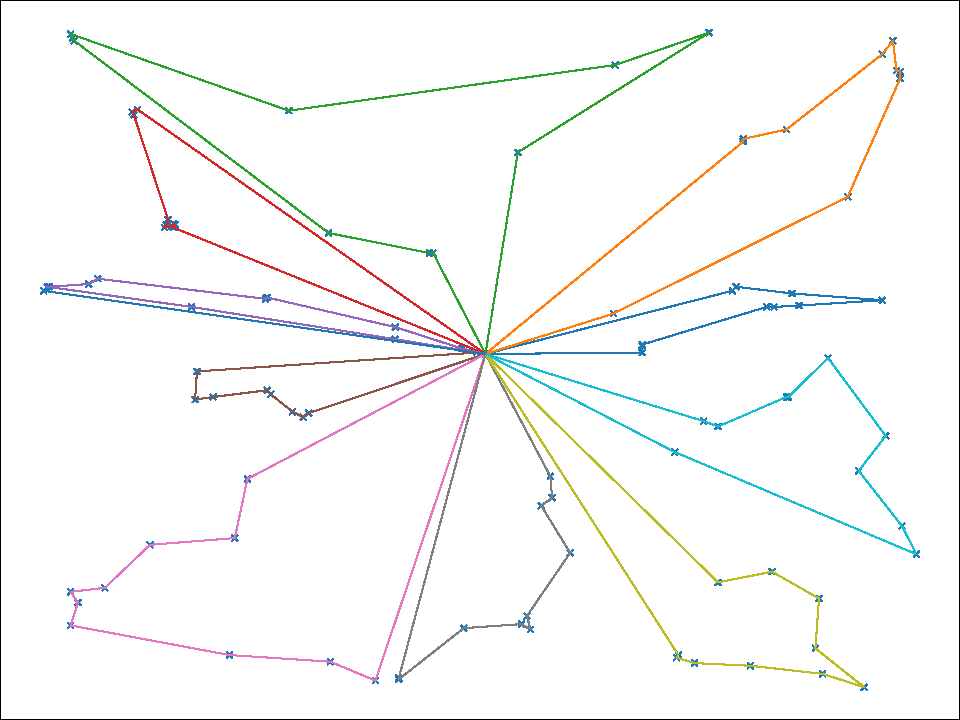
\includegraphics[width=0.45\textwidth]{images/TSAVN算法结果可视化.pdf}
    \caption{基于TSAVN的多无人机任务分配算法仿真结果}
    \label{fig:基于TSAVN的多无人机算法仿真结果}
\end{figure}

\subsection{算法性能对比实验结果}

为了直观地体现TSAVN算法的优越性,本节统计了性能测试中得到的性能指标,具体结果如表~\ref{tab:任务分配算法性能比较结果}所示。

\begin{table}[!htbp]
    \caption{任务分配算法性能比较结果}
    \label{tab:任务分配算法性能比较结果}
    \centering
    \begin{tabular}{c c c c c c c}
        \toprule
        \multirow{2}{*}{\textbf{运行次数}} & \multicolumn{2}{c}{\textbf{GA}} & \multicolumn{2}{c}{\textbf{SA}} & \multicolumn{2}{c}{\textbf{TSAVN}} \\
        \cmidrule(lr){2-3} \cmidrule(lr){4-5} \cmidrule(lr){6-7}
        & \makecell{运行时间\\(秒)} & 目标值 & \makecell{运行时间\\(秒)} & 目标值 & \makecell{运行时间\\(秒)} & 目标值 \\
        \midrule
        1 & 2086.7 & 66764.45 & 222.1 & 20759.26 & 9.731 & 18172.71\\
        2 & 1189.4 & 55713.22 & 204.2 & 19708.96 & 9.690 & 17882.67\\
        3 & 1181.4 & 52783.19 & 319.3 & 19358.90 & 9.155 & 17812.66\\
        4 & 1185.5 & 52623.57 & 127.6 & 20409.14 & 8.901 & 18052.71\\
        5 & 1182.3 & 55103.41 & 533.7 & 19009.00 & 8.200 & 17772.66\\
        6 & 1179.9 & 53380.95 & 541.9 & 18658.84 & 9.291 & 17962.69\\
        7 & 1177.1 & 55751.29 & 142.6 & 20059.25 & 9.759 & 17862.59\\
        8 & 1176.2 & 54941.32 & 205.4 & 19709.03 & 9.200 & 17772.56\\
        9 & 1179.6 & 53533.34 & 213.9 & 19708.96 & 9.119 & 18222.80\\
        10 & 1185.5 & 53222.29 & 167.2 & 20059.34 & 8.725 & 17542.58\\
        \textbf{平均值} & 1272.370 & 55381.703 & 267.790 & 19744.068 & \textbf{9.1771} & \textbf{17905.663} \\
        \bottomrule
    \end{tabular}
\end{table}

根据表~\ref{tab:任务分配算法性能比较结果}的试验结果,在目标值方面,本文所提出的TSAVN算法相较其他对比算法,得到的解质量更好,这体现了本文TSAVN在解决基于城市交通侦察场景下的无人机任务分配问题的有效性;在运行时间方面,本文算法相较其他对比算法而言同样有着更少的平均计算时间。综上所述,本文的TSAVN算法与其他算法相比具有显著的优越性。

\section{本章小结}

本章主要对本文所提出的任务计算资源的调度优化算法、多无人机航迹规划及任务分配算法在仿真环境下与不同的算法进行了性能测试,并进行了本文提出的算法与不同的算法在算法求解、运算时间等方面进行了性能的比较,进而得到本文所提出的算法的有效性及优越性。

\newpage
